\chapter{Introduction}
\label{chapter:introduction}

%\section{Background}

{\color{red}
(ideas) Include here the Problem Definition: details about the problem at hand (possibly in the same chapter as introduction)
}

{\color{red}
Action anticipation is a technique used in collaborative assembly to help robots and other autonomous systems predict the actions of their human collaborators and respond accordingly. By anticipating the actions of the human, the robot can better coordinate its own movements and actions to work efficiently and safely with the human. For example, if a human is reaching for a particular tool, the robot can anticipate this action and move to provide the tool to the human, or move out of the way to avoid a potential collision. This can help to improve the overall speed and efficiency of the collaborative assembly process, while also reducing the risk of accidents or injuries.
}

{\color{red}
(guide) The concept of Human-Robot Collaboration (HRC) involves the study of processes in which humans and robots work together to achieve a shared goal. Research on collision avoidance, human-aware planning of robot motions and control of physical contact have brought significant advances to the field of HRC. However, an essential requirement in the control of collaborative actions is the ability to anticipate the partner’s movements and intentions. The robot should not only be able to model and predict the human’s movements but, more importantly, must anticipate them. This dissertation proposal aims to tackle these questions using state-of-the-art Machine Learning (ML) techniques.
}

{\color{red}
(ideas) Include here definitions of anticipation, distinction between anticipation and recognition,...
}

%\section{Objectives}

{\color{red}
(guide) This dissertation aims at the development of an action anticipation system to enhance human-robot collaboration in industrial settings (see Fig.1) under the AUGMANITY mobilizing project. The main tasks to be carried out can be summarized by the following points:
\begin{itemize}
\item Overview of the state-of-the-art. To provide an up-to-date review of the definitions and algorithms adopted for action anticipation in collaborative environments.
\item Action anticipation in a human-robot collaborative scenario. To formally define how to anticipate an action in the context of the collaborative task under study using RGB-D images as input. ML models, such as recurrent neural networks (RNNs), are at the forefront of the algorithms to explore.
\item Robot control of joint actions. To develop anticipatory robot controllers that consider the human partner movements and intentions and use these inferences to make appropriate decisions during the execution of a sequential assembly task.
\item Metrics and performance evaluation. To provide performance metrics used to evaluate the action anticipation models and the add-value of the anticipatory controller (e.g., in terms of cycle time).
\item Writing the master dissertation and other detailed documentation.
\end{itemize}
}

{\color{red} 
\section{...from the article...}

% industrial rev
The Third Industrial Revolution was characterized by a focus on automating repetitive and heavy tasks on the assembly lines. Still, this created a problem: whenever the manufacturers needed the robots to work in a different assembly process, they needed to be reprogrammed by an expert.

The Fourth Industrial Revolution, also known as Industry 4.0, refers to the current trend of the manufacturing sector to become more intelligent and achieve greater automation. This trend takes advantage of the recent developments in artificial intelligence, the Internet of Things, and autonomous robots to pave the way for more efficient and flexible production processes. With Industry 4.0, robots are expected to be more adaptable and perform more actions without constant explicit programming. 

%HRC + cobots
Human-Robot Collaboration (HRC) aims to achieve greater efficiency by using robots in the same workspace as humans taking advantage of the strong points of both of them. These are called Collaborative Robots or Cobots and have significant benefits when working with people. For once, they can safely work with people since they have sensitive sensors that can detect the human interrupting them, causing them to stop their actions. They are also smaller, compact, and easy to program, among other advantages.\cite{CobotsWW}

One of the sub-fields of Human-Robot Collaboration is Human Action Anticipation which is the focus of this review.

\subsection{Definition of Anticipation}
 
 In Robotics, we can find a similar definition such as in \cite{Canuto2021}: "Action anticipation consists of classifying an action even before it occurs, by using the partial information provided up to a certain moment in time.".

 From these definitions, human action anticipation in HRC can be considered as the robot predicting the future actions of the human worker before he does them and then reacting accordingly.

To better visualize the real-world application, suppose, for example, that a human worker needs a specific material, such as a wooden plank. In this case, the robot can anticipate it and either provide it as it did in Fig.~\ref{example} or move out of the way to avoid a collision. Furthermore, anticipating human actions helps improve the overall speed and manufacturing efficiency of the collaborative assembly while also helping to reduce the risk of accidents or injuries, increasing safety.

\begin{figure}[htbp]
\centerline{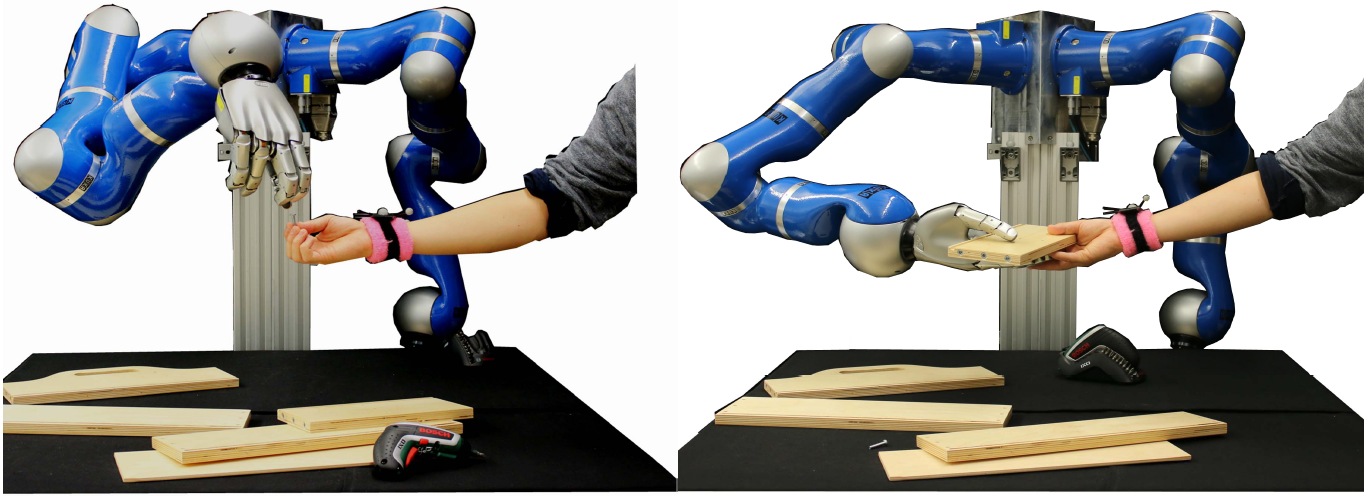
\includegraphics[width=3.5in]{figs/example.PNG}}
\caption{Situation where a robot anticipates that the worker will need a wooden plank and hands it over to him \cite{Maeda2016}}
\label{example}
\end{figure}

\subsection{Article Structure}

An action anticipation problem can be divided into three sub-problems. First, it must be decided which data needs to be captured by the sensors, then which algorithms should be used to analyze the captured data, and finally, how to increase the safety of the user. This division is also used to structure this article.
}